
\documentclass[notes]{beamer}       % print frame + notes
%\documentclass[notes=only]{beamer}   % only notes
% Replace the \documentclass declaration above
% with the following two lines to typeset your 
% lecture notes as a handout:
%\documentclass{article}
%\usepackage{beamerarticle}
\usetheme{default}
\usepackage{helvet}
\usepackage[compatibility=false]{caption}
\usepackage{subcaption}
\usepackage{multicol}
\usepackage{hyperref}
\usepackage{textcomp}
\usepackage{gensymb}
\usepackage{verbatim}



\usepackage{horacio}



% Default fixed font does not support bold face
\DeclareFixedFont{\ttb}{T1}{txtt}{bx}{n}{12} % for bold
\DeclareFixedFont{\ttm}{T1}{txtt}{m}{n}{12}  % for normal

% Custom colors
\usepackage{color}
\definecolor{deepblue}{rgb}{0,0,0.5}
\definecolor{deepred}{rgb}{0.6,0,0}
\definecolor{deepgreen}{rgb}{0,0.5,0}

\usepackage{listings}

% Python style for highlighting
\newcommand\pythonstyle{\lstset{
        language=Python,
        basicstyle=\ttm,
        otherkeywords={self},             % Add keywords here
        keywordstyle=\ttb\color{deepblue},
        emph={MyClass,__init__},          % Custom highlighting
        emphstyle=\ttb\color{deepred},    % Custom highlighting style
        stringstyle=\color{deepgreen},
        frame=tb,                         % Any extra options here
        showstringspaces=false            % 
}}


% Python environment
\lstnewenvironment{python}[1][]
{
    \pythonstyle
    \lstset{#1}
}
{}

% Python for external files
\newcommand\pythonexternal[2][]{{
        \pythonstyle
\lstinputlisting[#1]{#2}}}

% Python for inline
\newcommand\pythoninline[1]{{\pythonstyle\lstinline!#1!}}





\usepackage{tikz}
\usepackage{wasysym}

\title{Introducci\'on a la Computaci\'on} 

\author{Horacio Caniza Vierci\\horacio.caniza@upa.edu.py}
\pgfdeclareimage[height=0.5cm]{logo}{./images/logo}
\logo{\pgfuseimage{logo}}

% Let's get started
\begin{document}

\begin{frame}
    \titlepage
\end{frame}

\begin{frame}{Outline}
    \tableofcontents
    % You might wish to add the option [pausesections]
\end{frame}

%\begin{enumerate}
%\item ?`Qu\'e es la computaci\'on? \emph{Computer Science} o \emph{Informatics}?
%\item Historia de la computaci\'on.
%\item Arquitectura de sistemas.
%\item Fundamentos matem\'aticos de la computaci\'on:\emph{Das Entscheidungsproblem}.
%\end{enumerate}

\section{Historia y Sistemas operativos}
%
%1 hr.
\begin{frame}
    \frametitle{?`Qu\'e es la computaci\'on?}
    Computaci\'on es:
    \begin{itemize}
        \item Una tarea con objetivo definido que requiera, se beneficie de o cree computadoras \cite{ACM1}
        \item Entonces... \pause
            \begin{itemize}
                \item Construir hardware y software \pause
                \item Sistemas inteligentes, Comunicaciones, Juegos.  
                \item $\ldots$
            \end{itemize}
    \end{itemize}
    \pause
    ?`Y la computadora? ?`Qu\'e es la computadora?
    \begin{itemize}
        \item Una computadora no computa (!`no hace aritm\'etica!) \pause
        \item Una computadora es un \emph{data handler}!
    \end{itemize}
\end{frame}

\begin{frame}{Historia}
    Babbage and the lot.
    Insert timeline of computation here and discuss each step
\end{frame}

\begin{frame}{Dise\~nemos una computadora humana}
    Tenemos 4 operarios de archivo: \pause
    \begin{enumerate}
        \item Lento, pero conoce todas las operaciones. \pause
        \item 10 veces m\'as r\'apido, pero solo sabe sumar. \pause
        \item 10 veces m\'as r\'apido, pero no sabe sumar. \pause
        \item 10 veces m\'as r\'apido, pero no sabe siquiera leer.\pause
    \end{enumerate}
    \textcolor{red}{Una computadora general!} 
\end{frame}

\begin{frame}
    \frametitle{Representaci\'on binaria, \emph{aka} Computers are stupid}
    \begin{itemize}
       \item Armemos un sistema con colores: Azul y Rojo.
       \item !`Ejercicio! 
           \begin{itemize}
               \item Dise\~nar un sistema para identificar cuartos en un hotel usando dos colores. Establecer los l\'imites.
           \end{itemize}
    \end{itemize}
\end{frame}

%1.5
\begin{frame}{Arquitectura de sistemas modernos}
    \begin{itemize}
        \item ''First Draft of a Report on the EDVAC`` primavera de 1945. \pause 
            (\emph{aka} Steve Jobs vend\'ia un producto de m\'as de 60 a\~nos.) \pause
        \item Cuatro partes:
            \begin{enumerate}
                \item La Unidad Aritm\'etico-L\'ogica (ALU): realiza las operaciones.\pause
                \item La Unidad de Control Central(CU): controla y sincroniza \pause
                \item La memoria (M): almacena datos e instrucciones \pause
                \item Dispositivos de Input/Output (IO)
            \end{enumerate}
    \end{itemize}
\end{frame}

% SO 1

\begin{frame}{La computadora moderna}
    \begin{itemize}
        \item Uno o m\'as procesadores
        \item Sonido (entrada y salida), video (posiblemente varios), conexi\'on a redes, autenticaci\'on $\ldots$
    \end{itemize}
    \pause
    Una capa de \emph{software} que presenta un modelo simplificado del \emph{hardware}:
    \begin{itemize} 
        \item Windows, Mac, Android, IOS, Blackberry OS. \pause
        \item GNU/Linux, GNU Hurd, Minix, Solaris, LynxOS, Hp UX, $\ldots$ \pause
        \item ?`Y las m\'aquinas en una f\'abrica?
    \end{itemize}
    \pause
    \textcolor{red}{Sistema Operativo}
\end{frame}


\begin{frame}
    \frametitle{El sistema operativo como m\'aquina extendida}
    \begin{itemize}
        \item?`C\'omo imprimimos en la pantalla? \pause
        \item La abstracci\'on es esencial para manejar la complejidad. \pause
        \item Varios niveles de abstracci\'on
    \end{itemize}
\end{frame}

\begin{frame}
    \frametitle{Bajo nivel: C\'odigo m\'aquina} 
        b8    21 0a 00 00   \#moving "!n" into eax \\
        a3    0c 10 00 06   \#moving eax into first memory location \\
        b8    6f 72 6c 64   \#moving "orld" into eax \\
        a3    08 10 00 06   \#moving eax into next memory location \\
        b8    6f 2c 20 57   \#moving "o, W" into eax
        a3    04 10 00 06   \#moving eax into next memory location \\
        b8    48 65 6c 6c   \#moving "Hell" into eax \\
        a3    00 10 00 06   \#moving eax into next memory location \\
        b9    00 10 00 06   \#moving pointer to start of memory location into ecx \\
        ba    10 00 00 00   \#moving string size into edx \\
        bb    01 00 00 00   \#moving "stdout" number to ebx \\
        b8    04 00 00 00   \#moving "print out" syscall number to eax \\
        cd    80            \#calling the linux kernel to execute our print to stdout \\
        b8    01 00 00 00   \#moving "sys\_exit" call number to eax \\
        cd    80            \#executing it via linux sys\_call \\
        \pause \par
        \textcolor{red}{Resultado} \pause Imprime 'Hello World' en pantalla.
\end{frame}

\begin{frame}
\frametitle{Bajo/Medio nivel: Ensamblador}
    org  0x100       \\
    mov  dx, msg      \\
    mov  ah, 9        \\
    int  0x21         \\
    mov  ah, 0x4c     \\
    int  0x21         \\
    msg  db 'Hello World', 0x0d, 0x0a, '$'   ; $-terminated message \\
    \pause \par
    \textcolor{red}{Resultado} \pause Imprime 'Hello World' en pantalla.
\end{frame}

\begin{frame}
\frametitle{Alto nivel: Python}
    print('Hello World') \\
\pause
\textcolor{red}{Resultado} \pause Imprime 'Hello World' en pantalla.
\end{frame}

\begin{frame}
    \frametitle{El sistema operativo como administrador de recursos}
    \begin{block}{Escenario}
        Estoy jugando Clash of Clans y suena el FaceTime. ?`Qu\'e pasa?
    \end{block}
    \pause
    Multiplexar (Del Latin \emph{Multi} - Muchos, \emph{plexos} - Lados, dobleces)
    \begin{itemize}
        \item Tiempo \pause
        \item Espacio
    \end{itemize}
\end{frame}

\begin{frame}
    Mi computadora:
    \begin{itemize}
        \item GNU/Linux Debian 8: \pause 420.000.000 millones de instrucciones.
        \item El costo estimado: \pause 19.000 Millones de US\$.  
    \end{itemize}
    ?`Y en perspectiva?
        url{http://www.informationisbeautiful.net/visualizations/million-lines-of-code/}
\end{frame}



\section{2. El sistema binario}
%\begin{frame}
    \frametitle{Sistemas de numeraci\'on}
    \begin{itemize}
        \item La aritm\'etica es una \emph{herramienta}\pause
        \item ?`Una herramienta pr\'actica?:
            \begin{itemize}
                \item ?`Un \'unico s\'imbolo s\'imbolo? \pause
                \item ?`Un s\'imbolo por cada caso? \pause
            \end{itemize}
    \end{itemize}
    \textcolor{red}{Un conjunto reducido de s\'imbolos y reglas de combinaci\'on}
    \begin{itemize}
        \item Hexadecimal: 16 s\'imbolos (0 - 9 y A-F)
        \item Octal: 8 s\'imbolos (0 - 7)
        \item Binario: 2 s\'imbolos(0 y 1)
    \end{itemize}
\end{frame}
\note{
    \begin{enumerate}
        \item A tool to represent the world. to show us what we see.
        \item Examples about gazelles. One, two, many?
        \item Using pebbles? It must be practical, otherwise what is it good for
    \end{enumerate}
    \begin{itemize}
        \item We represent numbers with an underscore and teh base. 
        \item We assume all numbers are base 10.
    \end{itemize}
}

\begin{frame}
    \frametitle{Construyendo n\'umeros}
    \begin{block}{El n\'umero $1024_{10}$}
        $1024 = 1*10^3 + \pause 0*10^2 + \pause 2*10^1 +  4*10^0 $
    \end{block}
\end{frame}


\begin{frame}
    \frametitle{Los sistemas son equivalentes}
    \begin{block}{De base $n$ a base 10}
        $a = a_{n}*b^n + a_{n-1}*b^{n-1} + \ldots + a_{0} * b^{0}$
    \end{block}
    \pause
    \begin{block}{De base 10 a base $n$}
        \begin{itemize}
            \item Dividir el n\'umero por $n$ (divisi\'on entera). Registrar el Resto en Hexadecimal.
            \item Repetir con el cociente hasta que sea $0$.
        \end{itemize}
    \end{block}
\end{frame}

\begin{frame}
    \begin{ejercicio}{}
        Convertir $937_{10}$ a:
        \begin{itemize}
            \item Binario
            \item Ternario
            \item Cuaternario
            \item Octal
            \item Hexadecimal
        \end{itemize}
    \end{ejercicio}
    \pause
    \begin{ejercicio}{}
        Convertir $5ADC_{16}$ a: (hay un truco)
        \begin{itemize}
            \item Decimal
            \item Binario
            \item Ternario
            \item Cuaternario
            \item Octal
        \end{itemize}
    \end{ejercicio}
\end{frame}


\begin{frame}
    \begin{ejercicio}{}
        Responder:
        \begin{enumerate}
            \item Con 8 d\'igitos binarios (\emph{i.e.} un byte):  ?`cual es el mayor n\'umero que puedo representar en decimal?
            \item ?`Cu\'antos valores decimales distintos puedo generar con un byte?
        \end{enumerate}
    \end{ejercicio}

    \pause
    \begin{enumerate}
        \item $2^n - 1$
        \item $2^n$
    \end{enumerate}

\end{frame}

\subsection{Nuestro operador de archivos}

\begin{frame}
    \frametitle{Nuestro operario que no sabe leer $\ldots$}
    \pause
    \begin{itemize}
        \item Puede mirar: Prendido/Apagado, Hay/NoHay, 1/0, $\ldots$ \\
        \item Cuantos numeros puedo representar con binario.
    \end{itemize}
\end{frame}


\note{
    \begin{itemize}
        \item So the guy cannot read. What does he do? He needs to be able to understand that 10 is bigger than 9, but he cannot read!
        \item But he can ``feel''. He can feel power comming and not comming. Can't I then not combine it?
        \item What about the water? Make the example for the water circuit.
    \end{itemize}
}

\begin{frame}
    \frametitle{L\'ogica binaria}
    \begin{itemize}
        \item En base a 4 operaciones l\'ogicas: and, or, not, xor
    \end{itemize}
\end{frame}

\note{
    \begin{itemize}
        \item At this point I will draw the truth tables on teh board.
        \item Show the different circuits that can implement the logic. Explain that a combination of these is necessary.
    \end{itemize}
}

\subsection{Representaci\'on de la informaci\'on}

\begin{frame}
    \begin{itemize}
        \item ?`C\'omo se comunica que hay un nuevo papa? \pause
        \item ?`C\'omo funcionan los sem\'aforos? \pause
    \end{itemize}
    Un vocabulario basado en un alfabeto reducido.
\end{frame} 


\begin{frame}
    \frametitle{Codificando la informaci\'on}
    \begin{itemize}
        \item ?`Qu\'e necesitamos? \pause \textcolor{red}{Un convenio} 
        \item Hay varios: ASCII ( American Standard Code for Information Interchange ), UNICODE, UTF-8, $ldots$
    \end{itemize}

    \begin{table}[]
    \centering
    \begin{tabular}{lll}
        Decimal & Binario  & Char \\
        0       & 00000000 & NULL \\
        1       & 00000001 & SOH  \\
        2       & 00000010 & STX  \\
        ...     &          &      \\
        127     & 11111111 & DEL 
    \end{tabular}
    \end{table}
\end{frame}

\note{
    \begin{itemize}
        \item Explain that we need to represnet data in various ways.
        \item ASCII is one of them. ASCII is based on teletype: a typewriter that sent stuff via a cable.Think WW2 technology.
            \begin{itemize}
                \item It does not include any formatting information, but rather plaintext only
                \item Also, it includes some control characters.
            \end{itemize}
        \item What could the problems be? What happens with spanish? Could we use spanish?
    \end{itemize}
}

\begin{frame}
    \frametitle{Texto codificado en ASCII}
    \begin{block}{Universidad Paraguayo Alemana}
        01010101 01101110 01101001 01110110 01100101 01110010 01110011 01101001 01100100 01100001 01100100 00100000 01010000 01100001 01110010 01100001 01100111 01110101 01100001 01111001 01101111 00100000 01000001 01101100 01100101 01101101 01100001 01101110 01100001 
    \end{block}
\end{frame}

\begin{frame}
    \begin{ejercicio}{}
    Decodificar la siguiente secuencia ASCII: \\
        01100101 01101110 00100000 01110011 01101001 01101100 01100101 01101110 01100011 01101001 01101111 00100000 01110011 01100001 01101100 01101001 01110010 00100000 01100001 01101100 00100000 01110010 01100101 01100011 01110010 01100101 01101111
    \end{ejercicio}
\end{frame}

\note{
    Print and copy an ascii table for the people.
}

\subsection{Aritm\'etica en binario}

\begin{frame}
    \frametitle{Suma}
    \begin{table}[]
    \centering
    \begin{tabular}{lll}
        A & B & + \\
        0 & 0 & 0\\
        0 & 1 & 1\\
        1 & 0 & 1\\
        1 & 1 & 10 \\
    \end{tabular}
    \end{table}

    Ejemplo:
    $1010_{2} + 11_{2} = 1101_{2}$
\end{frame}

\begin{frame}
    \frametitle{Resta}
    La resta es m\'as compleja. Hay dos m\'etodos
    \begin{table}[]
    \centering
    \begin{tabular}{lll}
        A & B & - \\
        1 & 1 & 0\\
        0 & 0 & 0\\
        1 & 0 & 1\\
        0 & 1 & 0 (habiendo acarreado de la siguiente posici\'on)\\
    \end{tabular}
    \end{table}
    Ejemplo:
    $1010_{2} - 11_{2} = 0111_{2}$
\end{frame}

\begin{frame}
    \frametitle{Resta 1}
    $1010_{2} - 11_{2} = 0111_{2}$
    \begin{itemize}
        \item $0 - 1 = 1$ 
        \item $0 - 1 = 1$ \pause
        \item $1 - 0 = 1$ \pause
        \item $0 - 0 = 1$ \pause
    \end{itemize}
\end{frame}

\note{
    \begin{itemize}
        \item No fue posible hacer 0 -1, entonces acarreamos del anterior. Vienen dos por la posicion.
        \item No podemos acarrear del cero, asique tenemosq ue ir hasta qeu podamos y volver.
    \end{itemize}
}


\begin{frame}
    \frametitle{Resta 2}
    \begin{enumerate}
        \item Completar la cantidad de digitos para igualar los n\'umeros con ceros. \emph{e.g.} 01010 - 011 $\rightarrow$ 01010 - 00011
        \item Sumar el complemento
        \item Si la \'ultima sma tiene excedente, sumar ese excedente al resultado.
   \end{enumerate}
   \pause
    $1010_{2} - 11_{2} = 1010_{2} + 1100_{2} = (1)0110_{2} = 0110_{2} + 1_{2} = 0111_{2}$
\end{frame}

\begin{frame}
    \begin{ejercicio}{}
    Sumar:
        \begin{enumerate}
            \item 11 + 1	
            \item 11 + 11	
            \item 111 + 11	
            \item 111 + 10	
            \item 1110 + 111	
            \item 1100 + 110	
            \item 1111 + 10101	
            \item 1100 + 11001	
            \item 1011 + 1101	
            \item 1110 + 10111	
            \item 1110 + 1111	
            \item 11111 + 11101	
        \end{enumerate}
    \end{ejercicio}
\end{frame}

\begin{frame}
    \begin{ejercicio}{}
        Restar:
        \begin{enumerate}
            \item 11 - 10	
            \item 110 - 10	
            \item 1111 - 110	
            \item 100 - 10	
            \item 100 - 11	
            \item 1000 - 11	
            \item 1101 - 110	
            \item 11011 - 110	
            \item 1111 - 111	
            \item 110101 - 1010	
            \item 11011 - 111	
            \item 11110 - 111
        \end{enumerate}
    \end{ejercicio}
\end{frame}

\begin{frame}
    \frametitle{Multiplicaci\'on}
    \begin{enumerate}
        \item Copiar el primer factor cuando multiplicado por 1. Sino, una fila de 0
        \item Desplazar una columna a la izquierda al mover al siguiente digito del segundo factor. Repetir.
        \item Sumar todos los valores.
    \end{enumerate}
\end{frame}

\note{
    Make example of multiplication
}

\begin{frame}
    \begin{ejercicio}{}
        Multiplicar
        \begin{enumerate}
            \item 11 * 1	
            \item 11 * 11	
            \item 111 * 11	
            \item 111 * 10	
            \item 1110 * 111	
            \item 1100 * 110	
            \item 1111 * 10101	
            \item 1100 * 11001	
            \item 1011 * 1101	
            \item 1110 * 10111	
            \item 1110 * 1111	
            \item 11111 * 11101	
        \end{enumerate}
    \end{ejercicio}
\end{frame}


\begin{frame}
    \frametitle{Uniendo los cabos}
    
\includegraphics[scale=0.25]{./images/adder.png}
    \\
    \vspace{10mm}
    \begin{center}
        \huge{\textcolor{red}{?}}
    \end{center}

\end{frame}

\begin{frame}
    \frametitle{Uniendo los cabos}
    \begin{columns}
        \begin{column}{0.5\textwidth}
            
\includegraphics[scale=0.15]{./images/adder.png}
        \end{column}
        \begin{column}{0.5\textwidth}
                \begin{table}[]
                \centering
                \begin{tabular}{llll}
                    A & B & x & C\\
                    0 & 0 & 0 & 0\\
                    0 & 1 & 1 & 0\\
                    1 & 0 & 1 & 0\\
                    1 & 1 & 0 & 1\\
                \end{tabular}
                \end{table}
        \end{column}
    \end{columns}
\end{frame}

\note{
    \begin{itemize}
        \item Hablamos de representar la informaci\'on utilizando notaci\'on binaria y las cuatro operaciones.
        \item Mencionamos una cantidad de operaciones. Pero como funciona esto en binario y usando 4 operaciones?
        \item A dise\~nar un circuito
        \item Maybe remove this?
    \end{itemize}
}

\subsection{Fundamentos matem\'aticos de la computaci\'on}

\begin{frame}
    \frametitle{Los algoritmos}
    \begin{block}{Informalmente}
        Una colecci\'on de instrucciones para realizar una tarea espec\'ifica.
    \end{block}
    \pause
    \begin{block}{Formalmente}
        Secuencia de operaciones que puede ser interpretada por un sistema Turing-completo.
    \end{block}
\end{frame}

\note{
    \begin{itemize}
        \item Example about showering.
    \end{itemize}
}

\begin{frame}
    \frametitle{Las capacidades fundamentales de los sistemas de computaci\'on}
    \begin{itemize}
        \item Aut\'omatas 
        \item Complejidad \pause
        \item Computabilidad \pause
    \end{itemize}
    o\\
    ?`Qu\'e podemos calcular?
\end{frame}

\note{
    Introduce the concept of algorithm. That is, a procedure that needs to be done following a specific set of 
    steps. Some might be interchanged, some may not
}

\begin{frame}
    \frametitle{Aut\'omatas}
    Modelos computacionales
    \begin{itemize}
        \item Abstraer del dispositivo de c\'omputo (?`La ALU?) \pause
        \item ?`El poder del modelo?
    \end{itemize}
\end{frame}

\note{
    \begin{itemize}
        \item We are trying to reason on the computer, without getting lost in the complexities of the machine.
        \item But, not all models are good models. Gravity and high speeds, for example. We cannot use newtonian mechanics
            to explain quantum effects.
        \item We'll analyse the one model: FA.
    \end{itemize}
}


\begin{frame}
    \frametitle{Aut\'omatas de estado finito}
    Modelemos una puerta autom\'atica.
\end{frame}

\note{
    \begin{itemize}
        \item What do we need? That is, which elements to we need: Sensor, Door, Motor and the controller for the motor.
        \item If we wish to abstract, what do we care about? The door opening when someone comes, and closing when they leave.
    \end{itemize}
}


\begin{frame}
    \frametitle{El FA como reconocedor de lenguajes}
    \begin{center}
        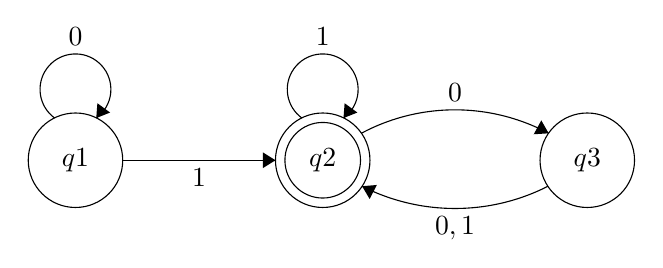
\begin{tikzpicture}[scale=0.2]
        \tikzstyle{every node}+=[inner sep=0pt]
        \draw [black] (16.4,-28.4) circle (3);
        \draw (16.4,-28.4) node {$q1$};
        \draw [black] (32.1,-28.4) circle (3);
        \draw (32.1,-28.4) node {$q2$};
        \draw [black] (32.1,-28.4) circle (2.4);
        \draw [black] (48.9,-28.4) circle (3);
        \draw (48.9,-28.4) node {$q3$};
        \draw [black] (15.077,-25.72) arc (234:-54:2.25);
        \draw (16.4,-21.15) node [above] {$0$};
        \fill [black] (17.72,-25.72) -- (18.6,-25.37) -- (17.79,-24.78);
        \draw [black] (19.4,-28.4) -- (29.1,-28.4);
        \fill [black] (29.1,-28.4) -- (28.3,-27.9) -- (28.3,-28.9);
        \draw (24.25,-28.9) node [below] {$1$};
        \draw [black] (30.777,-25.72) arc (234:-54:2.25);
        \draw (32.1,-21.15) node [above] {$1$};
        \fill [black] (33.42,-25.72) -- (34.3,-25.37) -- (33.49,-24.78);
        \draw [black] (34.554,-26.687) arc (118.10792:61.89208:12.62);
        \fill [black] (46.45,-26.69) -- (45.98,-25.87) -- (45.5,-26.75);
        \draw (40.5,-24.7) node [above] {$0$};
        \draw [black] (46.404,-30.052) arc (-63.08675:-116.91325:13.043);
        \fill [black] (34.6,-30.05) -- (35.08,-30.86) -- (35.54,-29.97);
        \draw (40.5,-31.96) node [below] {$0,1$};
        \end{tikzpicture}
    \end{center}
    \begin{ejercicio}{}
        ?`Cu\'al es el conjunto de cadenas reconocido por este FA?
    \end{ejercicio}
\end{frame}

\begin{frame}
    \begin{ejercicio}{}
        Dise\'~nar un FA que reconozca la letra ``A'' codificada en ASCII.
    \end{ejercicio}
\end{frame}

\begin{frame}
    \frametitle{Definici\'on formal de un FA}
    Un FA es una 5-tupla:
    \begin{enumerate}
        \item $Q$ es un conjunto finito de estados.
        \item $\Sigma$ es un conjunto finito de car\'acteres, el alfabeto.
        \item $\delta:Q \times \Sigma \rightarrow Q$ es la funci\'on de transici\'on.
        \item $F \subseteq Q$ un conjunto de estados de aceptaci\'on.
    \end{enumerate}
\end{frame}


\begin{frame}
    \begin{center}
        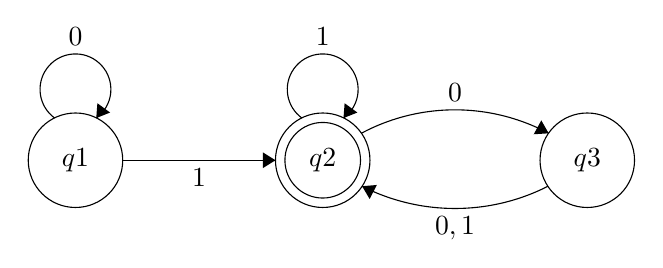
\begin{tikzpicture}[scale=0.2]
        \tikzstyle{every node}+=[inner sep=0pt]
        \draw [black] (16.4,-28.4) circle (3);
        \draw (16.4,-28.4) node {$q1$};
        \draw [black] (32.1,-28.4) circle (3);
        \draw (32.1,-28.4) node {$q2$};
        \draw [black] (32.1,-28.4) circle (2.4);
        \draw [black] (48.9,-28.4) circle (3);
        \draw (48.9,-28.4) node {$q3$};
        \draw [black] (15.077,-25.72) arc (234:-54:2.25);
        \draw (16.4,-21.15) node [above] {$0$};
        \fill [black] (17.72,-25.72) -- (18.6,-25.37) -- (17.79,-24.78);
        \draw [black] (19.4,-28.4) -- (29.1,-28.4);
        \fill [black] (29.1,-28.4) -- (28.3,-27.9) -- (28.3,-28.9);
        \draw (24.25,-28.9) node [below] {$1$};
        \draw [black] (30.777,-25.72) arc (234:-54:2.25);
        \draw (32.1,-21.15) node [above] {$1$};
        \fill [black] (33.42,-25.72) -- (34.3,-25.37) -- (33.49,-24.78);
        \draw [black] (34.554,-26.687) arc (118.10792:61.89208:12.62);
        \fill [black] (46.45,-26.69) -- (45.98,-25.87) -- (45.5,-26.75);
        \draw (40.5,-24.7) node [above] {$0$};
        \draw [black] (46.404,-30.052) arc (-63.08675:-116.91325:13.043);
        \fill [black] (34.6,-30.05) -- (35.08,-30.86) -- (35.54,-29.97);
        \draw (40.5,-31.96) node [below] {$0,1$};
        \end{tikzpicture}
    \end{center}
    \begin{enumerate}
        \item $Q = \left\{q1, q2, q3\right\}$
        \item $\Sigma = \left\{1,0\right\}$
        \item $\delta:Q \times \Sigma \rightarrow Q = ((q1,0),q1), ((q1,1),q2),\ldots$
        \item $F \subseteq Q = \left\{q2\right\}$ 
    \end{enumerate}
\end{frame}

\begin{frame}
    \begin{center}
        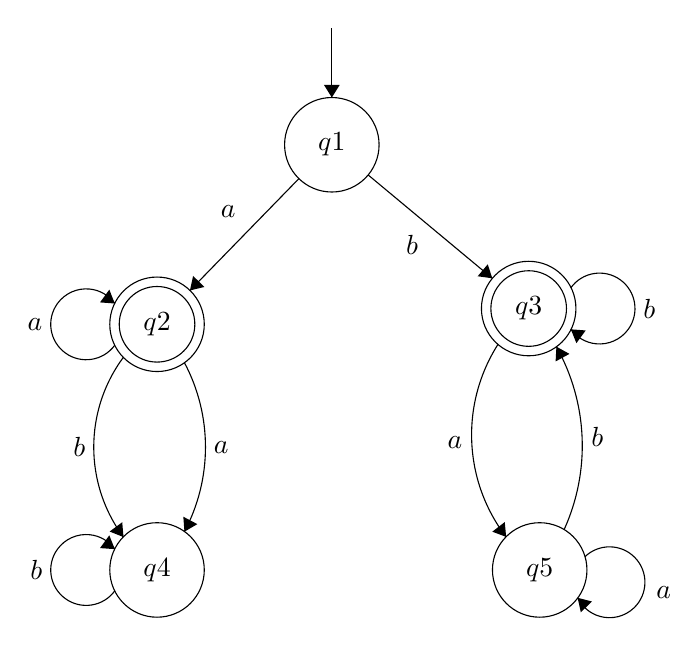
\begin{tikzpicture}[scale=0.2]
        \tikzstyle{every node}+=[inner sep=0pt]
        \draw [black] (36.3,-12.7) circle (3);
        \draw (36.3,-12.7) node {$q1$};
        \draw [black] (25.2,-24.1) circle (3);
        \draw (25.2,-24.1) node {$q2$};
        \draw [black] (25.2,-24.1) circle (2.4);
        \draw [black] (48.8,-23.1) circle (3);
        \draw (48.8,-23.1) node {$q3$};
        \draw [black] (48.8,-23.1) circle (2.4);
        \draw [black] (25.2,-39.7) circle (3);
        \draw (25.2,-39.7) node {$q4$};
        \draw [black] (49.5,-39.7) circle (3);
        \draw (49.5,-39.7) node {$q5$};
        \draw [black] (36.3,-5.3) -- (36.3,-9.7);
        \fill [black] (36.3,-9.7) -- (36.8,-8.9) -- (35.8,-8.9);
        \draw [black] (22.52,-25.423) arc (324:36:2.25);
        \draw (17.95,-24.1) node [left] {$a$};
        \fill [black] (22.52,-22.78) -- (22.17,-21.9) -- (21.58,-22.71);
        \draw [black] (22.52,-41.023) arc (-36:-324:2.25);
        \draw (17.95,-39.7) node [left] {$b$};
        \fill [black] (22.52,-38.38) -- (22.17,-37.5) -- (21.58,-38.31);
        \draw [black] (34.21,-14.85) -- (27.29,-21.95);
        \fill [black] (27.29,-21.95) -- (28.21,-21.73) -- (27.49,-21.03);
        \draw (30.22,-16.93) node [left] {$a$};
        \draw [black] (23.067,-37.608) arc (-143.42715:-216.57285:9.579);
        \fill [black] (23.07,-37.61) -- (22.99,-36.67) -- (22.19,-37.26);
        \draw (20.68,-31.9) node [left] {$b$};
        \draw [black] (26.938,-26.534) arc (28.0065:-28.0065:11.426);
        \fill [black] (26.94,-37.27) -- (27.76,-36.79) -- (26.87,-36.32);
        \draw (28.78,-31.9) node [right] {$a$};
        \draw [black] (38.61,-14.62) -- (46.49,-21.18);
        \fill [black] (46.49,-21.18) -- (46.2,-20.29) -- (45.56,-21.05);
        \draw (41.39,-18.39) node [below] {$b$};
        \draw [black] (51.48,-21.777) arc (144:-144:2.25);
        \draw (56.05,-23.1) node [right] {$b$};
        \fill [black] (51.48,-24.42) -- (51.83,-25.3) -- (52.42,-24.49);
        \draw [black] (47.369,-37.602) arc (-142.60752:-212.56317:10.678);
        \fill [black] (47.37,-37.6) -- (47.28,-36.66) -- (46.49,-37.27);
        \draw (44.62,-31.58) node [left] {$a$};
        \draw [black] (50.559,-25.522) arc (29.29843:-24.46912:12.856);
        \fill [black] (50.56,-25.52) -- (50.51,-26.46) -- (51.39,-25.98);
        \draw (52.75,-31.26) node [right] {$b$};
        \draw [black] (52.369,-38.863) arc (133.99202:-154.00798:2.25);
        \draw (56.87,-41.13) node [right] {$a$};
        \fill [black] (51.91,-41.47) -- (52.11,-42.39) -- (52.82,-41.7);
        \end{tikzpicture}
    \end{center}

    \begin{ejercicio}{}
            Especificar el FA en la figura. Definir el lenguaje.
    \end{ejercicio}
\end{frame}

\begin{frame}
    \begin{center}
        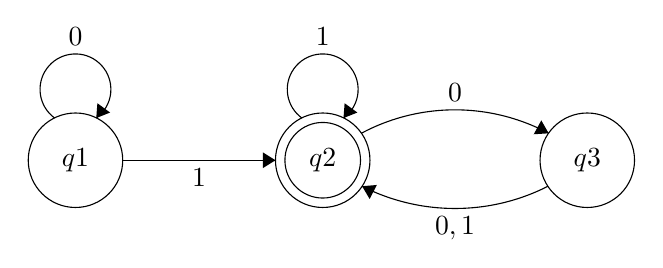
\begin{tikzpicture}[scale=0.2]
        \tikzstyle{every node}+=[inner sep=0pt]
        \draw [black] (16.4,-28.4) circle (3);
        \draw (16.4,-28.4) node {$q1$};
        \draw [black] (32.1,-28.4) circle (3);
        \draw (32.1,-28.4) node {$q2$};
        \draw [black] (32.1,-28.4) circle (2.4);
        \draw [black] (48.9,-28.4) circle (3);
        \draw (48.9,-28.4) node {$q3$};
        \draw [black] (15.077,-25.72) arc (234:-54:2.25);
        \draw (16.4,-21.15) node [above] {$0$};
        \fill [black] (17.72,-25.72) -- (18.6,-25.37) -- (17.79,-24.78);
        \draw [black] (19.4,-28.4) -- (29.1,-28.4);
        \fill [black] (29.1,-28.4) -- (28.3,-27.9) -- (28.3,-28.9);
        \draw (24.25,-28.9) node [below] {$1$};
        \draw [black] (30.777,-25.72) arc (234:-54:2.25);
        \draw (32.1,-21.15) node [above] {$1$};
        \fill [black] (33.42,-25.72) -- (34.3,-25.37) -- (33.49,-24.78);
        \draw [black] (34.554,-26.687) arc (118.10792:61.89208:12.62);
        \fill [black] (46.45,-26.69) -- (45.98,-25.87) -- (45.5,-26.75);
        \draw (40.5,-24.7) node [above] {$0$};
        \draw [black] (46.404,-30.052) arc (-63.08675:-116.91325:13.043);
        \fill [black] (34.6,-30.05) -- (35.08,-30.86) -- (35.54,-29.97);
        \draw (40.5,-31.96) node [below] {$0,1$};
        \end{tikzpicture}
    \end{center}

    \begin{ejercicio}{}
            Especificar el FA en la figura. Definir el lenguaje.
    \end{ejercicio}
\end{frame}

\note{
    Hasta ahora no hablamos de nada mas que el FA. Es decir, el model oque estamos explroando es simple, pero mostramos que 
    puede hacer varias cosas. Puede reconocer letras, puede reconocer patrones, etc. \\
    Tiene poca memoria, como se codifica la memoria? Como piensan que se representa la memoria?
}

\subsection{Definici\'on formal de Computaci\'on. Propiedades de los FA}

\begin{frame}
    \frametitle{Computaci\'on}
    Sea $M = \left(Q,\Sigma, \delta, q_{0}, F\right)$ un FA. Sea $w = w_{1}w_{2}, \ldots, w_{n}$
    una cadena donde $w_{i} \in \Sigma, 0 < i \leq n$. $M$ acepta $w$ si existe una secuencia
    de estados $r_{0},r_{1}, \ldots, r_{m}$  con $r_{i} \in Q, 0 \leq i \leq m $ si:
    \begin{itemize}
        \item $r_{0} = q_{0}$
        \item $\delta(r_{i}, w_{i+1}) = r_{i+1}, 0 \leq i \leq m$
        \item $r_{n} \in F$
    \end{itemize}
    \begin{itemize}
        \item $L\left(M\right)$ es el conjunto de cadenas que acepta $M$.  
        \item $M$ reconoce el lenguaje $A$ si $A = \left\{w | w \in L\left(M\right)\right\}$
    \end{itemize}
    Un lenguaje $A$ es \emph{regular} si existe un FA que lo reconozca.
\end{frame}

\begin{frame}
    \begin{block}{Si yo digo}
        Para contar necesito memoria infinita. ?`Es verdad o mentira?
    \end{block}
    \pause
    \begin{center}
        Es verdad y es mentira.  Depende del modelo. \smiley. 
    \end{center}
\end{frame}

\begin{frame}
    \begin{ejercicio}{}
        Construir un FA que reconozca la siguiente cadena: 111000.\pause
    \end{ejercicio}
    \begin{ejercicio}{}
        Construir un FA que reconozca las siguientes cadenas: $1^n0^n$
    \end{ejercicio}
\end{frame}

\note{
    No se puede! Hacer notar que es la misma cantidad de 1 que de 0. Porque decimos storage infinito>?
    porque si tuvieramos infinitos estados podemos construir todos los posibles combinaciones de iguales. 
}

\begin{frame}
    \frametitle{El pumping lemma}
    Formalmente:
    Si $w \in A$, y $|w| > |Q|$, entonces: \\
    \vspace{2mm}
    $\exists q\in Q~y~x \in \Sigma^{+}$ tal que:
    \begin{enumerate}
        \item $w = yxz$
        \item $\delta^*(q,x) = q$
    \end{enumerate}
    entonces: $yx^nz \in A \forall n \geq 0$\\
    \pause
    Informalmente:\\
    Si existe una cadena en un lenguaje reconocido por un FA que pueda ser descompuesta en tres partes: $y,x,z$ tal que $x$ empiece y termine 
    en el mismo estado, entonces el FA va a reconocer cualquier cadena con un n\'umero arbitrario de $x$.
\end{frame}


\begin{frame}
    \huge{\textcolor{red}{Un FA no puede contar}}
\end{frame}

\note{
    Here we prove it.
    \begin{itemize}
        \item It is not that we say the FA is crap, but rather, an insufficient model. We need to use something more powerful
    \end{itemize}
}

\begin{frame}
    \frametitle{Para hacer en casa}
    \begin{itemize}
        \item Challenge 1 - Números Binarios
        \item Challenge 2 - Demostraci\'on.
    \end{itemize}This 
\end{frame}


\section{3. Lenguajes de programaci\'on: Conceptos}
\begin{frame}
\frametitle{Lenguajes de programaci\'on}
    \begin{itemize}
        \item Un lenguaje formal  \pause
        \item Dise\~nado para comunicar instrucciones a la m\'aquina \pause
        \item Para expresar algoritmos. \pause
    \end{itemize}
    \emph{ Un leguaje regular!}
\end{frame}


\begin{frame}
    \frametitle{Algoritmos}
    Un procedimiento:
    \begin{itemize}
        \item Las acciones a ejecutar
        \item El \'orden
    \end{itemize}
\end{frame}

\note{
    La ducha. El orden es importante.
}

\begin{frame}
    \frametitle{El lenguaje de programaci\'on Python}
    Dos grupos grandes:
    \begin{itemize}
        \item Compilados: C, C++, C\#, $\ldots$
        \item Interpretados: Ruby, Bash, Perl, Python, $\ldots$
    \end{itemize}
    Python es un lenguaje \emph{orientado a objetos} interpretado.
\end{frame}


\note{
    What is the difference between these two languages:
    \begin{itemize}
        \item Does not need to be built
        \item Interpretetd is much much slower
        \item Compilation defines the machine.
    \end{itemize}
    Explain object orientation
}

\begin{frame}
    \frametitle{Python es}
    \begin{enumerate}
        \item Simple
        \item Es ``Free'' as in freedom, not ``free'' beer. \pause
        \item Es de alto nivel \pause
        \item Portablo \pause
        \item Interpretado \pause
        \item Orientado a objetos \pause
        \item Extensible \pause
    \end{enumerate}
\end{frame}

\subsection{Instalando Python}

\begin{frame}
    \begin{enumerate}
        \item Vamos a usar Python  en su versi\'on 3
        \item Vamos a usar jupyter notebook: Usamos el navegador como editor
    \end{enumerate}
\end{frame}

\begin{frame}
    \frametitle{Instalando python}
    \begin{itemize}
        \item Instalar Anaconda (una distribuci\'on de python. Incluye muchas cosas) 
        \item \url{https://www.continuum.io/downloads} (Bajar la version 3.5)
    \end{itemize}
    Instalar jupyter notebook
    \begin{itemize}
        \item Abrir una terminal (En Mac: Utilities->Applications, en Windows: Tecla Win + R, en GNU/Linux)
        \item coda install jupyter
    \end{itemize}
\end{frame}


\begin{frame}
    \frametitle{Probemos nuestro editor y nuestro lenguaje}
    \begin{itemize}
        \item Abrir una terminal (En Mac: Utilities->Applications, en Windows: Tecla Win + R, en GNU/Linux)
        \item jupyter notebook
    \end{itemize}
\end{frame}


\begin{frame}[fragile]
\frametitle{El primer programa}
\begin{python}
    print 'Hello World!'
\end{python}
Para ejecutar, apretar \texttt{Shift} y \texttt{Enter}.
\end{frame}


\begin{frame}
    \frametitle{Modos de operaci\'on de python}
    \begin{itemize}
        \item Interactivo \pause
        \item Script.
    \end{itemize}
\end{frame}

\begin{frame}
    \frametitle{Interactivo}
    \begin{itemize}
        \item Cada sentencia o conjunto de setencias es independiente
            \begin{itemize}
                \item En la consola: ejecutar \texttt{python}
                \item En el notebook
            \end{itemize}
    \end{itemize}
\end{frame}

\begin{frame}
    \frametitle{Script}
    \begin{itemize}
        \item Todas las sentencias se eval\'uan en conjunto
            \begin{itemize}
                \item Crear el programa en un archivo
                \item Cambiar la extensi\'on a \texttt{.py}
                \item Ejecutar el script: \texttt{python <archivo>.py}
            \end{itemize}
    \end{itemize}
\end{frame}

\subsection{Variables, expresiones y tipos}

\begin{frame}
    \begin{enumerate}
        \item Valor y tipo \pause
        \item Variables \pause
        \item Operaciones \pause
    \end{enumerate}
\end{frame}


\note{
    \begin{itemize}
        \item A esto hacemos detalle. explicamos el concepto de tipo de dato. 
        \item Enlazar con al representacion binaria de los datos 
        \item Mencionar las clases, mencionar que todos los tipos son clases y que por lo tanto son extensibles. El concepto de clase mencionamos rapidamente.
        \item Tenemos que mencionar que pasa con las variables y las operaciones. Sumar cadenas? Sumar enteros? dividir enteros? Representacion de numeros.
        \item Mencionar que no todos los elementos son identificaroes de variables validos.
        \item Explicar que hay tipos de variables que son fijos en otros lenguajes.
    \end{itemize}
}

\begin{frame}[fragile]
    Dado:
    \begin{python}
        a = 2
        b = 2.0
        c = '.'
    \end{python}
    Que resulta de:
    \begin{python}
        a/3
        b/3
        b + c
    \end{python}
\end{frame}

\begin{frame}[fragile]
    \frametitle{Cadenas}
    \begin{itemize}
        \item Una cadena es una \emph{sequencia} de car\'acteres.
        \item Uno puede referirse a un car\'acter en particular, empezando a 0 hasta n - 1
        \item La longitud de la cadena se mide con \texttt{len}
            \begin{python}
                a = 'horacio'
                print a[0]
                print len(a)
            \end{python}
    \end{itemize}
    \begin{python}
        print a[1.3]
        print a[10]
    \end{python}
\end{frame}


\begin{frame}[fragile]
    \frametitle{Condiciones}
    Si quiero indicar condiciones:
    \begin{itemize}
        \item La palabra clave \textbf{if} seguida de la condici\'on:
            \begin{python}
                if temperatura == 45:
                    print 'Hace mucho calor'
            \end{python}
    \end{itemize}
\end{frame}

\begin{frame}
    \frametitle{Ejercicios}
    \begin{enumerate}
        \item Resultado de \texttt{2 / 3} es 0. ?`Por qu\'e?
        \item Calcular la distancia que recorre una persona que corre a 12 km/h en 2.4 horas.
        \item Tigo me ofrece 100Gb. de datos a 10Mbps. Si bajo constantemente datos a la maxima velocidad, 
            ?`En cuanto tiempo llego al l\'imite? (10 Mbps son 10.000.000 bits segundo. 100 Gb son 100.000.000.000.000 bits)
        \item El vol\'umen de una esfera esta dado por $\frac{4}{3}\pi r^3$ donde r es el radio. Calcular.
    \end{enumerate}
\end{frame}

\begin{frame}
    \vspace{15mm}
    Lista de ejercicios: Ej_introduccion.pdf (\emph{en el classroom})
\end{frame}


\subsection{Estructuras de control}


\subsection{Estructuras de datos}


\begin{frame}
    \frametitle{Listas}
\end{frame}


\begin{frame}[fragile]
    \frametitle{Funciones}
    Una funci\'on es un conjunto de setencias que realiza una tarea espec\'ifica.
    \begin{python}
        def calcular_volumen(radio):
            return (4/3)*3.14*(r**3)
    \end{python}
\end{frame}

\begin{frame}
    \frametitle{Ciclos}
\end{frame}

\note{
    Definir el concepto de bloque en python y como los espacios determinan esto.\\
    Explicar las partes de la funcion.

}

\begin{frame}
    \frametitle{Ejercicios}
    \begin{enumerate}
        \item Definir el procedimiento histograma() que produce in histograma. Por ejemplo, histograma(1) es *, histograma(3) es ***
        \item Definir una funci\'on reverso(cadena) que invierte una cadena. Por ejemplo reverso('horacio') es 'oicaroh'
        \item Definir una funci\'on capicua(nombre) que retorna 'Si' si nombre es capicua. Una palabra capicua se lee de ambos lados igual, por ejemplo Anana
        \item Escribir una funci\'on que compute la longitud de una cadena sin usar la funci\'on len.
        \item Definir una funci\'on que suma los elementos de una lista.
        \item Definir una funci\'on que multiplica los elementos de una lista.
    \end{enumerate}
\end{frame}

\begin{frame}
    \frametitle{Tarea para la casa:}
    Leer el cap\'itulo 1.
\end{frame}


\section{4. Lenguajes de programaci\'on: Sentencias, procedimientos y funciones}

\section{5. \LaTeX}
% Generalidades del Tex
%
\begin{frame}{\LaTeX}
    \begin{block}{¿Qu\'e es \TeX ?}
        Es un lenguaje creado por Donald E. Knuth. 
    \end{block}
    \begin{block}{¿Qu\'e es \LaTeX{}?}
        \LaTeX{} es un paquete de \emph{macros} o funciones escrito por Leslie Lamport.
    \end{block}
\end{frame}


\begin{frame}{Psst..?`Qu\'e es \LaTeX realmente?}
    \begin{itemize}
        \item Una herramienta creada por nerds para nerds.
            \begin{itemize}
                \item Dif\'icil de usar.\pause
                \item M\'as lenta para empezar.\pause
                \item Cuando uno quiere hacer cosas chicas, es una p\'erdida de tiempo.\pause
            \end{itemize}
            \textcolor{red}{Peero..} tiene aspectos positivos \pause\\
            \begin{itemize}
                \item Es dif\'icil de usar.
                \item Produce documentos incomparables.
                \item Permite manejar las diferentes versiones.
                \item Para documentos grandes es la \'unica herramienta realmente.
            \end{itemize}
    \end{itemize}
\end{frame}

%%%%%%%%%%%%%%%%

% ¿Cómo funciona?
%\begin{frame}{Generalidades}
%	\begin{block}{¿Cómo funciona?}
%	Generalmente, a la hora de publicar un texto, el \emph{autor} envía su manuscrito a la editorial. El \emph{maquetador} decide el aspecto del documento (anchura de columnas, tipografía, espacios,...). El maquetador manda estas instrucciones al \emph{compositor}, quien compone el libro de acuerdo a tales instrucciones.
%	
%	En un entorno \LaTeX{}, \LaTeX{} representa el papel del maquetador y usa \TeX{} como su compositor. Pero \LaTeX{} es sólo un programa y por tanto necesita que el autor proporcione información para describir la estructura lóqica de su trabajo. Estas informaciones se conocen como “órdenes \LaTeX{}”.
%	\end{block}
%\end{frame}

% Producción de textos estructurados
\begin{frame}{Generalidades}
    \begin{block}{Producci\'on de textos estructurados.}
        \vspace{-.4cm}
        \begin{multicols}{2}
            \begin{figure}
                \centering
                \begin{subfigure}[b]{0.5\textwidth} 
                    \centering
                    \includegraphics[scale=.04]{images/autor}
                    \caption{El autor}			
                \end{subfigure}

                \vspace*{.25cm}			

                \begin{subfigure}[b]{0.5\textwidth} 
                    \centering
                    \includegraphics[scale=.08]{images/maquetador}
                    \caption{El maquetador}
                \end{subfigure}

                \vspace*{.25cm}				

                \begin{subfigure}[b]{0.5\textwidth} 
                    \centering
                    \includegraphics[scale=.12]{images/compositor}
                    \caption{El compositor}
                \end{subfigure}
            \end{figure}	
            \newpage

            \vspace*{.50cm}
            $\rightarrow$ env\'ia su manuscrito a la editorial (al maquetador). 

            \vspace*{.70cm}
            $\rightarrow$ recibe el manuscrito del autor y decide el aspecto del documento y env\'ia instrucciones al compositor.

            \vspace*{.50cm}
            $\rightarrow$ recibe las instrucciones del maquetador y compone el libro en base a tales instrucciones.
        \end{multicols}
    \end{block}
\end{frame}
%%%%%%%%%%%%%%%%

%Producción de textos estructurados con LaTeX
\begin{frame}{Generalidades}
    \begin{block}{Producci\'on de textos estructurados en \LaTeX{}.}
        \vspace{-.4cm}
        \begin{multicols}{2}
            \begin{figure}
                \centering
                \begin{subfigure}[b]{0.5\textwidth} 
                    \centering
                    \includegraphics[scale=.08]{images/autor_LaTeX}
                    \caption{El autor}			
                \end{subfigure}

                \vspace*{.25cm}			

                \begin{subfigure}[b]{0.5\textwidth} 
                    \centering
                    \includegraphics[scale=.09]{images/maquetador_LaTeX}
                    \caption{El maquetador}
                \end{subfigure}

                \vspace*{.25cm}				

                \begin{subfigure}[b]{0.5\textwidth} 
                    \centering
                    \includegraphics[scale=.06]{images/compositor_LaTeX}
                    \caption{El compositor}
                \end{subfigure}
            \end{figure}	
            \newpage

            \vspace*{.05cm}
            $\rightarrow$ Escribe el texto y \textbf{proporciona informaci\'on para describir la estructura l\'ogica de su trabajo}.


            \vspace*{.70cm}
            $\rightarrow$ interpreta la informaci\'on proveída por el autor y env\'ia las directrices al compositor.

            \vspace*{.90cm}
            $\rightarrow$ recibe las instrucciones de \LaTeX{} y compone el libro.
        \end{multicols}
    \end{block}
\end{frame}
%%%%%%%%%%%%%%%%


\begin{frame}{Generalidades}
    \begin{block}{\LaTeX{} vs MS Word}
        \begin{figure}
            \centering
            \includegraphics[scale=.3]{images/LaTeX_vs_Word.pdf}
        \end{figure}
        \begin{center}
            Si es dif\'icil de aprender vale la pena.
        \end{center}
    \end{block}
\end{frame}
%%%%%%%%%%%%%%%%

\section{Probando...}
\begin{frame}{Probando el funcionamiento}
    \begin{block}{Serie de instrucciones}
        \textbackslash documentclass[10pt,a4paper]\{article\} \\
        \textbackslash usepackage[utf8]\{inputenc\} \\
        \textbackslash begin\{document\} \\
        \textbackslash section\{Hola Mundo!\} \\
        Bienvenido al mundo de \textbackslash LaTeX \\
        \textbackslash end\{document\}
    \end{block}
\end{frame}

%%%%%%%%%%%%%%%%

\section{Archivos de entrada \LaTeX{}}

\begin{frame}{Archivos de entrada}
    \begin{itemize}
        \item \emph{Varios caracteres consecutivos} en blanco se tratan como un \emph{solo} ``espacio''. 
        \item Espacios en blanco al principio de una l\'inea se ignoran y un salto de l\'inea aislado se trata como ``espacio''
    \end{itemize}
    \begin{exampleblock}{Ejercicio 01}
        Escribir la palabra ``Hola'' seguida de 10 espacios blancos y luego ``Mundo''.
    \end{exampleblock}
    \begin{exampleblock}{Ejercicio 02}
        Escribir la palabra ``Hola'' seguida de 10 quiebres de linea (la tecla Enter) y luego ``Mundo''.
    \end{exampleblock}
\end{frame}
%%%%%%%%%%%%%%%%

\begin{frame}{Archivos de entrada \LaTeX{}}
    Son s\'imbolos reservados:
    \begin{itemize}
        \item \# \hspace*{1em} \$ \hspace*{1em} \% \hspace*{1em} \^{} \hspace*{1em} \& \hspace*{1em} \_ \hspace*{1em} \{ \hspace*{1em} \} \hspace*{1em} \~{} \hspace*{1em} $\backslash$
        \item Para que \LaTeX{} imprima estos s\'imbolos debemos escribir: \\
            $\backslash$\# \hspace*{.7em} $\backslash$\$ \hspace*{.7em} $\backslash$\% \hspace*{.7em} $\backslash$\^{}\{\} \hspace*{.7em} $\backslash$\& \hspace*{.7em} $\backslash$\_ \hspace*{.7em} $\backslash$\{ \hspace*{.7em} $\backslash$\} \hspace*{.7em} $\backslash$\~{}\{\} \hspace*{.7em} \$$\backslash$backslash\$
        \item Para imprimir acentos: \\ seguidos del tipo de acento (' o \textasciitilde). 
    \end{itemize}
    \begin{exampleblock}{Ejercicio 03}
    Generar correctamente la siguiente salida en \LaTeX{}: \\ \# $\backslash$ \$ \& $\backslash$ 	\} \{
    \end{exampleblock}
\end{frame}
%%%%%%%%%%%%%%%

\begin{frame}{Archivos de entrada \LaTeX{}}
    \begin{block}{Ordenes \LaTeX{}}
        Las \'ordenes \LaTeX{} son sensibles a may\'usculas, y adoptan uno de los formatos siguientes:
        \begin{itemize}
            \item Comienzan con una barra invertida $\backslash$ y luego tienen un nombre que consiste sólo en letras. 
                Los nombres de orden terminan con un espacio
            \item Consisten en una barra invertida y exactamente una no letra.
        \end{itemize}	
    \end{block}

    \begin{exampleblock}{Ejercicio 04}
        Probar que $\backslash$TeX $\backslash$LaTeX produce lo mismo que $\backslash$TeX$\backslash$LaTeX
    \end{exampleblock}	
    %	\begin{exampleblock}{Ejercicio 05}
    %		Probar que $\backslash$\# $\backslash$\$ \textbf{NO} produce lo mismo que $\backslash$\#$\backslash$\$
    %	\end{exampleblock}
\end{frame}
%%%%%%%%%%%%%%%%%

\begin{frame}{Archivos de entrada \LaTeX{}}
    \begin{block}{Comentarios}
        Cuando \LaTeX{} encuentra un caracter \% prescinde el resto de la l\'inea actual, 
        el salto de l\'inea y todo el espacio en blanco al comienzo de la l\'inea siguiente.
    \end{block}
    \begin{exampleblock}{Ejercicio 05}
        Probar:\\
        Este es un \% est\'upido \\
        \% REALMENTE ESTÚPIDO \\
        \hspace{2cm} ejemplo de c\'omo se puede usar el \% \\
        \hspace{1cm} s\'imbolo de comentario.
    \end{exampleblock}
\end{frame}
%%%%%%%%%%%%%%%%

\section{Estructura del archivo de entrada}

\begin{frame}{Estructura del fichero de entrada}
    \begin{block}{Partes del fichero de entrada}
        \textbf{TODO} documento escrito en \LaTeX{} consta de dos partes: \textbf{el pr\'eambulo} y el \textbf{cuerpo del texto}.
        \begin{itemize}
            \item El pr\'eambulo \textbf{siempre} empieza por la orden \\
                \texttt{$\backslash$documentclass\{...\}} \\
                Esto indica que tipo de documento se pretende escribir. 
                Luego de definir el tipo de documento se establecen los paquetes a utilizar \\
                \texttt{$\backslash$usepackage\{...\}}
            \item El cuerpo del texto comienza con la orden
                \texttt{$\backslash$begin\{document\}} \\
                Al final del documento \\
                \texttt{$\backslash$end\{document\}}\\
                Cualquier cosa que preceda esta última orden será ignorada por \LaTeX{}.
        \end{itemize}
    \end{block}
\end{frame}

\begin{frame}
    \begin{block}{Serie de instrucciones}
        \textbackslash documentclass[10pt,a4paper]\{article\} \\
        \textbackslash usepackage[utf8]\{inputenc\} \\
        \textbackslash begin\{document\} \\
        \textbackslash Hola Mundo!\\
        Bienvenido al mundo de \textbackslash LaTeX \\
        \textbackslash end\{document\}
    \end{block}
\end{frame}
%%%%%%%%%%%%%%%%

\section{El aspecto del documento}

\begin{frame}{El aspecto del documento}
\begin{block}{Clases de documento}
Esto se indica con la orden \texttt{$\backslash$documentclass}.\\
\texttt{$\backslash$documentclass[opciones]\{clase\}} \\
\emph{clase} indica el tipo de documento, con \emph{opciones} para personalizar.
    \end{block}

    \begin{exampleblock}{Ejemplo 01}
        Un archivo de entrada para un documento \LaTeX{} podría empezar con la l\'inea\\
        \texttt{$\backslash$documentclass[11pt,twoside,a4paper]\{article\}}
    \end{exampleblock}			
\end{frame}
%%%%%%%%%%%%%%%

\begin{frame}{Clases de documentos}
\begin{itemize}
    \item \texttt{article}, \texttt{minimal}, \texttt{report}, \pause
    \item \texttt{beamer:} para la producción de diapositivas \textbf{(Esta clase se utiliz\'o para preparar estos slides.)}
\end{itemize}
\end{frame}
%%%%%%%%%%%%%%%

\begin{frame}{Opciones de clases de documentos}
Hay muchas opciones.
\begin{itemize}
    \item Tama\~no de letra \item \texttt{10pt, 11pt, 12pt} \pause
    \item Tama\~no de papel \item \texttt{a4paper, letterpaper,...} \pause
    \item $\ldots$
\end{itemize}
\end{frame}
%%%%%%%%%%%%%%%

\begin{frame}{Paquetes}
    Los paquetes se incluyen. Son librer\'ias de c\'odigo \TeX\\
    \texttt{$\backslash$usepackage[opciones]\{paquete\}}\\

    \begin{alertblock}{Información sobre paquetes}
        Si tienen alguna duda sobre un paquete: Nombre del Paquete + "latex" en google.
    \end{alertblock}
\end{frame}
%%%%%%%%%%%%%%%

\begin{frame}{Estilos de p\'agina}
    \begin{block}{Tipos de estilo}
        \LaTeX{} soporta tres combinaciones predifinidas de cabeceras y pies de página, llamadas estilos de p\'agina. \\
        \texttt{$\backslash$pagestyle\{estilo\}} \\
        Los estilos son:
        \begin{itemize}
            \item \texttt{plain} imprime los n\'umeros de página en la parte de abajo, en el centro del pie. 
            \item \texttt{headings} imprime el nombre del capítulo actual y el n\'umero de p\'agina en la cabecera de cada p\'agina, mientras que el pie queda vac\'io.
            \item \texttt{empty} sin cabecera ni pie de p\'agina.
        \end{itemize}
        Para cambiar el estilo: \\
        \texttt{$\backslash$thispagestyle\{estilo\}}
    \end{block}
\end{frame}
%%%%%%%%%%%%%%%

\section{Proyectos grandes}

\begin{frame}{Proyectos grandes}
    Cuando se trabaja en proyectos grandes, dividir el archivo en partes.
    \texttt{$\backslash$include\{nombre-de-fichero\}}\\
    \texttt{$\backslash$include} agrega una nueva l\'inea.\\
    Para evitar esta nueva l\'inea:\\
    \texttt{$\backslash$input\{nombre-de-fichero\}}
\end{frame}
%%%%%%%%%%%%%%%

\section{Usemos \LaTeX}

\begin{frame}{Ejercicio 06}
    Copiar dos cap\'itulo del Tao of programming (disponible en el classroom) con el formato siguiente:
\end{frame}
%%%%%%%%%%%%%%%

\begin{frame}{Ejercicio 06}
    \begin{exampleblock}{Especificaciones requeridas}
        \begin{itemize}
            \item Clase de documento: art\'iculo
            \item Opciones de clases de documento: 
                \begin{itemize}
                    \item Letra 11pt
                    \item Papel A4
                    \item A dos columnas
                \end{itemize}
        \end{itemize}
    \end{exampleblock}

\end{frame}
%%%%%%%%%%%%%%%

\begin{frame}{Ejercicio 06}
    \begin{exampleblock}{Consideraciones importantes}
        \begin{itemize}
            \item Para crear el título del documento utiliza la orden \texttt{$\backslash$title\{t\'itulo\}} y en el pre\'ambulo.
                Luego escribe la orden \texttt{$\backslash$maketitle} al incio del cuerpo del texto.
            \item Para crear un resumen:\\
                \texttt{$\backslash$begin\{abstract\}} \\
                \textit{Escribir el resumen} \\
                \texttt{$\backslash$end\{abstract\}}
            \item Para crear una secci\'on usa la orden \texttt{$\backslash$section\{...\}}
            \item Para crear una subsecci\'on usa la orden \texttt{$\backslash$subsection\{...\}}
        \end{itemize}
    \end{exampleblock}
\end{frame}
%%%%%%%%%%%%%%%

\section{Saltos de l\'inea y p\'agina}

\begin{frame}{Saltos de l\'inea y de p\'agina}
    \begin{block}{Justificaci\'on de p\'arrafos}
        \begin{itemize}
            \item Salte de l\'inea con: \texttt{$\backslash\backslash$} o \texttt{$\backslash$newline}
            \item Salto forzado de página: \texttt{$\backslash$newpage}
            \item La orden: \texttt{$\backslash\backslash$*} \\ prohibe que exista un salto de p\'agina tras el salto forzado de l\'inea.
        \end{itemize}
    \end{block}
\end{frame}
%%%%%%%%%%%%%%%

\begin{frame}{Saltos de l\'inea y de p\'agina}
    \begin{block}{Evitar separaciones}
        \begin{itemize}
            \item A veces es necesario mantener un argumento sin que se separe.  \texttt{$\backslash$mbox\{...\}} 
        \end{itemize}
    \end{block}
\end{frame}
%%%%%%%%%%%%%%%

\begin{frame}{Saltos de l\'inea y de p\'agina}
    \begin{exampleblock}{Ejercicio 07}
        \begin{itemize}
            \item Genera la siguiente salida: \\
                Este es un ejemplo \\
                de c\'omo \newline
                realizar saltos de \\
                l\'inea.
            \item Genera la siguiente salida: \\
                \fbox{Este es un ejemplo del uso de $\backslash$fbox}
            \item Genera la siguiente salida sin que se silabe el n\'umero de cuenta:\\
                El n\'umero de cuenta en la que debes realizar el dep\'osito es 123 456 789 555 000, puedes pasar esta tarde por el banco.
        \end{itemize}
    \end{exampleblock}
\end{frame}
%%%%%%%%%%%%%%%

\section{S\'imbolos}

    \begin{frame}{Comillas}
        Para generar comillas no se debe usar \textbf{"}. En tipograf\'ia hay comillas especiales de apertura y cierre.\\
        En \LaTeX{}, se utilizan dos acentos graves para abrir comillas y dos ap\'ostrofes para cerrar comillas. \\
        Para comillas simples basta con un ap\'ostrofe.

        \begin{exampleblock}{Ejercicio 08}
            \begin{itemize}
                \item Genere las siguientes salidas: \\
                    ``Este es un ejemplo del correcto uso de comillas'' \\
                    \fbox{Estoy aprendiendo a usar ``\LaTeX{}''. ¡Odio este tema!}\\
                    Ahora ya aprend\'i que el comando \fbox{``\%''} se utiliza para hacer 'comentarios'. 	
             \end{itemize}
        \end{exampleblock}
    \end{frame}
    %%%%%%%%%%%%%%%

    \begin{frame}{Guiones y rayas}
        En \LaTeX{} existen cuatro tipos distintos de gui\'on:

        \begin{block}{¿Cómo obtenerlos?}
            \begin{itemize}
                \item Guión ``-''
                \item Raya corta ``--''
                \item Raya ``---''
            \end{itemize}

        \end{block}
        El resto de los s\'imbolos? Mirar el archivo LatexSimbols.pdf en el classroom.
    \end{frame}
    %%%%%%%%%%%%%%%
    %%%%%%%%%%%%%%%

    \section{T\'itulos, cap\'itulos y secciones}

    \begin{frame}{T\'itulos, cap\'itulos y secciones}

        Las siguientes \'ordenes estan disponibles para la clase \texttt{article}: \\
        \begin{itemize}
            \item \texttt{$\backslash$section\{...\}} \\
            \item \texttt{$\backslash$subsection\{...\}} \\
            \item \texttt{$\backslash$subsubsection\{...\}} \\
            \item \texttt{$\backslash$paragraph\{...\}} \\
            \item \texttt{$\backslash$subparagraph\{...\}}
        \end{itemize}
        Si se quiere dividir el documento en partes sin influir la numeraci\'on de secciones o capítulos se puede usar:
        \begin{itemize}
            \item \texttt{$\backslash$part\{...\}}
        \end{itemize}
    \end{frame}
    %%%%%%%%%%%%%%%

    \begin{frame}
        \frametitle{Indices}
        Para crear un \'indice:
        \begin{itemize}
            \item \texttt{$\backslash$tableofcontents}
        \end{itemize}
        y ubica el índice general en el lugar donde se ejecuta la orden.

        \begin{alertblock}{¡Ojo!}
            Todas las comandos de secci\'on tienen una versi\'on ``estrella'' seguidas de un asterisco (\texttt{$\backslash$section\{...\}*}).
                Generan encabezados de secci\'on pero no aparecen en el \'indice y no se enumeran.
        \end{alertblock}

        \begin{alertblock}{Títulos muy largos}
            Si un encabezado es muy largo:
            \texttt{$\backslash$section[T\'itulo para el \'indice general]\{Un largo y aburrido t\'itulo que va a a aparecer en el texto. \}}
        \end{alertblock}

    \end{frame}
    %%%%%%%%%%%%

    \begin{frame}
        \begin{block}{T\'itulo general}
            El t\'itulo de todo el documento se genera:
            \begin{itemize}
                \item  \texttt{$\backslash$maketitle}
            \end{itemize}
            El contenido del t\'itulo tiene que definirse en el pre\'ambulo:
            \begin{itemize}
                \item \texttt{$\backslash$title\{...\}}
                \item \texttt{$\backslash$author\{...\}}
                \item \texttt{$\backslash$date\{...\}}
            \end{itemize}

            En el argumento \texttt{$\backslash$author} se pueden poner varios nombres separado por \texttt{$\backslash$and}
        \end{block}

        \begin{exampleblock}{Ejercicio 10}
            \begin{itemize}
                \item Generar el \'indice general y completar los datos de autor y fecha para el texto del Ejercicio 06.
            \end{itemize}
        \end{exampleblock}
    \end{frame}
    %%%%%%%%%%%%%%%

    \section{Notas al pie}

    \begin{frame}{Notas al pie}
        Con la orden \\
        \texttt{$\backslash$footnote\{\emph{texto al pie}\}} \\
        se imprime una nota al pie en la p\'agina actual. 
            
        \begin{exampleblock}{Ejercicio 11}
            \begin{itemize}
                \item Escriba una nota al pie en el texto del Ejercicio 06 para comprobar su funcionamiento.
            \end{itemize}
        \end{exampleblock}

    \end{frame}

    \section{Estilos de letra}

    \begin{frame}{Estilos de letra}
        \begin{block}{Los distintos estilos}
            \LaTeX{} tiene varios estilos de letra que pueden ser utilizados, ellos son: \\
            \begin{itemize}
                \item \textbf{Negrita} \texttt{$\backslash$textbf\{...\}}
                \item \textit{Cursiva} \texttt{$\backslash$textit\{...\}}
                \item \texttt{M\'aquina de escribir} \texttt{$\backslash$texttt\{...\}}
                \item \emph{Enfasis} \texttt{$\backslash$emph\{...\}}
            \end{itemize}
        \end{block}

        \begin{exampleblock}{Ejercicio 12}
            \begin{itemize}
                \item Genere la siguiente salida. \\
                    Yo estudio \textbf{Ingenier\'ia Industrial} \textit{estar\'ia bueno saber} en que ``met\'i''. \\
            \end{itemize}
        \end{exampleblock}
    \end{frame}



\begin{frame}[allowframebreaks]
  \frametitle<presentation>{Referencias}
    
  \begin{thebibliography}{10}
    
  \beamertemplatebookbibitems
  % Start with overview books.

  \bibitem{ACM1}
      The Joint Task Force for Computing Curricula 2005
    \newblock {Computing Curricula 2005}.
    \newblock ACM and IEEE 2005
 
    
  \beamertemplatearticlebibitems
  % Followed by interesting articles. Keep the list short. 

  \bibitem{Someone2000}
    S.~Someone.
    \newblock On this and that.
    \newblock {\em Journal of This and That}, 2(1):50--100,
    2000.
  \end{thebibliography}
\end{frame}


\end{document}


